\section{Foreword}
There has been a few things I've been uncertain about with this assignment. First, I wasn't sure exactly \textbf{how} I was supposed to show the success of some of the steps (unpacked images for example -- unpacking these is a \textit{dependency} for the other steps, as is logging into Kali). Second, I am not sure if I interpreted \textit{Access services on the other hosts - including authentication attempts} correctly. The way I interpreted this is \textit{booting} these images and making sure they work.
It could also have been interpreted as \textit{getting access to} the systems these images contain. The reason I interpreted it as such was because it said \textit{authentication \textbf{attempts}}, and because running a vulnerability scanner was optional. Scanning would probably have been the first thing I tried if this was supposed to mean gaining access to these systems - the motd in these systems speak against this however, but I made the assumptions that rooting them is part of upcoming assignments.

I have also chosen to use VirtualBox over VMware because I see no reason for proprietary software when there's a fully qualified open source equivalent.

\section{Set-up}

Alright, so let's get going -- I will use screenshots and code snippets to make every step I took as clear as possible.

% Unpack images

\subsection{Downloading and unpacking images}

\hspace*{-5in}\begin{lstlisting}[language=bash,caption={Unpacking images}]
[amnesthesia@vngr Assignments]$ mkdir EthHack
[amnesthesia@vngr Assignments]$ cd EthHack
[amnesthesia@vngr EthHack]$ wget http://www.kioptrix.com/dlvm/Kioptrix_Level_1.rar

--2014-09-05 12:54:25--  http://www.kioptrix.com/dlvm/Kioptrix_Level_2.rar
Resolving www.kioptrix.com (www.kioptrix.com)... 72.55.186.61
Connecting to www.kioptrix.com (www.kioptrix.com)|72.55.186.61|:80... connected.
HTTP request sent, awaiting response... 200 OK
Length: 424883454 (405M) [application/x-rar-compressed]
Saving to: 'Kioptrix_Level_2.rar'

[amnesthesia@vngr EthHack]$ wget http://www.kioptrix.com/dlvm/Kioptrix_Level_2.rar
--2014-09-05 12:53:45--  http://www.kioptrix.com/dlvm/Kioptrix_Level_1.rar
Resolving www.kioptrix.com (www.kioptrix.com)... 72.55.186.61
Connecting to www.kioptrix.com (www.kioptrix.com)|72.55.186.61|:80... connected.
HTTP request sent, awaiting response... 200 OK
Length: 194624731 (186M) [application/x-rar-compressed]
Saving to: 'Kioptrix_Level_1.rar'

[amnesthesia@vngr EthHack]$ unrar x Kioptrix_Level_1.rar
Extracting from Kioptrix_Level_1.rar

Creating    Kioptix Level 1                                   OK
Extracting  Kioptix Level 1/Kioptix Level 1.nvram             OK 
Extracting  Kioptix Level 1/Kioptix Level 1.vmdk              OK 
Extracting  Kioptix Level 1/Kioptix Level 1.vmsd              OK 
Extracting  Kioptix Level 1/Kioptix Level 1.vmx               OK 
Extracting  Kioptix Level 1/Kioptix Level 1.vmxf              OK

[amnesthesia@vngr EthHack]$ unrar x Kioptrix_Level_2.rar
Extracting from Kioptrix_Level_2.rar

Creating    Kioptrix Level 2                                  OK
Extracting  Kioptrix Level 2/CentOs4.5.nvram                  OK 
Extracting  Kioptrix Level 2/CentOs4.5.vmdk                   OK 
Extracting  Kioptrix Level 2/CentOs4.5.vmsd                   OK 
Extracting  Kioptrix Level 2/CentOs4.5.vmx                    OK 
Extracting  Kioptrix Level 2/CentOs4.5.vmxf                   OK

\end{lstlisting}

\section{Network}
I set up a VirtualBox Host Adapter with a DHCP-server.\\
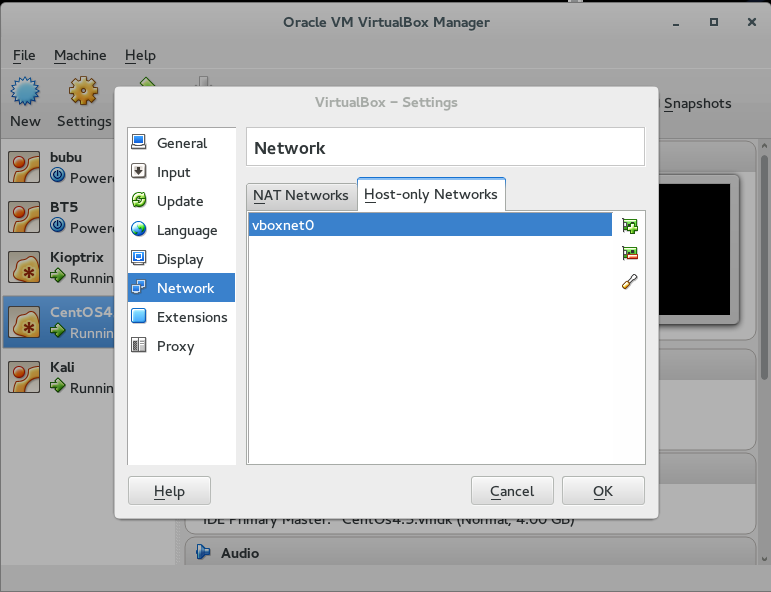
\includegraphics[scale=0.5]{nw.png}

\subsection{Creating a VirtualBox Host Adapter}
The host's adapter is located at \textit{192.168.56.2}, and the DHCP server is located at \textit{192.168.56.2}. This leaves \textit{192.168.56.3-254} available for the DHCP IP pool, with 255 as the broadcast address.\\

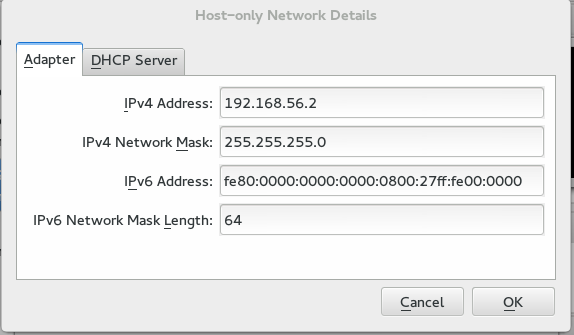
\includegraphics[scale=0.7]{nw_adapter.png}\\

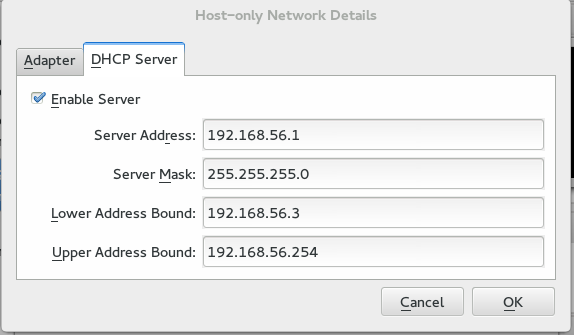
\includegraphics[scale=0.7]{nw_dhcp.png}\\

As can be seen by the ifconfig output in Kali, Kali was assigned IP 102 on this network. I'd say this sufficiently explains why this IP is private (assuming that by private you mean host-only?), as this network is virtual and run between the VMs.

\begin{lstlisting}[language=bash,caption={Kali IP-address}]
root@battlestation:~# ifconfig
eth0	Link encap:Ethernet HWaddr: 08:00:27:9f:c1:c6
		inet addr:192.168.56.102 Bcast:192.168.56.255
\end{lstlisting}

I'm not entirely sure how "nmap scan" is any different from "scan for other hosts" either, but here we go!
% Scan for other hosts
\begin{lstlisting}[language=bash,caption={Network scan}]

Starting Nmap 6.46 ( http://nmap.org ) at 2014-09-05 11:45 CEST
NSE: Loaded 118 scripts for scanning.
NSE: Script Pre-scanning.
Initiating ARP Ping Scan at 11:45
Scanning 254 hosts [1 port/host]
Completed ARP Ping Scan at 11:45, 2.43s elapsed (254 total hosts)
Initiating Parallel DNS resolution of 254 hosts. at 11:45
Completed Parallel DNS resolution of 254 hosts. at 11:45, 13.00s elapsed
Nmap scan report for 192.168.56.1 [host down]
[...]
Initiating Parallel DNS resolution of 1 host. at 11:45
Completed Parallel DNS resolution of 1 host. at 11:46, 13.00s elapsed
Initiating SYN Stealth Scan at 11:46
Scanning 4 hosts [1000 ports/host]
Discovered open port 139/tcp on 192.168.56.101
Discovered open port 111/tcp on 192.168.56.101
Discovered open port 111/tcp on 192.168.56.103
Discovered open port 443/tcp on 192.168.56.101
Discovered open port 443/tcp on 192.168.56.103
Discovered open port 22/tcp on 192.168.56.101
Discovered open port 3306/tcp on 192.168.56.103
Discovered open port 3306/tcp on 192.168.56.104
Discovered open port 22/tcp on 192.168.56.103
Discovered open port 80/tcp on 192.168.56.101
Discovered open port 80/tcp on 192.168.56.103
Discovered open port 32768/tcp on 192.168.56.101
Discovered open port 902/tcp on 192.168.56.104
Discovered open port 631/tcp on 192.168.56.103
Completed SYN Stealth Scan against 192.168.56.101 in 0.34s (3 hosts left)
Completed SYN Stealth Scan against 192.168.56.103 in 0.34s (2 hosts left)
Completed SYN Stealth Scan against 192.168.56.104 in 0.34s (1 host left)
Completed SYN Stealth Scan at 11:46, 3.36s elapsed (4000 total ports)
Initiating Service scan at 11:46
Scanning 14 services on 4 hosts
Completed Service scan at 11:46, 12.06s elapsed (14 services on 4 hosts)
Initiating OS detection (try #1) against 4 hosts
Retrying OS detection (try #2) against 2 hosts
Retrying OS detection (try #3) against 192.168.56.104
Retrying OS detection (try #4) against 192.168.56.104
Retrying OS detection (try #5) against 192.168.56.104
NSE: Script scanning 4 hosts.
Initiating NSE at 11:46
Completed NSE at 11:46, 3.08s elapsed
Nmap scan report for 192.168.56.100
Host is up (0.00016s latency).
All 1000 scanned ports on 192.168.56.100 are filtered
MAC Address: 08:00:27:1F:11:E9 (Cadmus Computer Systems)
Too many fingerprints match this host to give specific OS details
Network Distance: 1 hop

TRACEROUTE
HOP RTT     ADDRESS
1   0.16 ms 192.168.56.100

Nmap scan report for 192.168.56.101
Host is up (0.00040s latency).
Not shown: 994 closed ports
PORT      STATE SERVICE     VERSION
22/tcp    open  ssh         OpenSSH 2.9p2 (protocol 1.99)
|_ssh-hostkey: ERROR: Script execution failed (use -d to debug)
|_sshv1: Server supports SSHv1
80/tcp    open  http        Apache httpd 1.3.20 ((Unix)  (Red-Hat/Linux) mod_ssl/2.8.4 OpenSSL/0.9.6b)
| http-methods: GET HEAD OPTIONS TRACE
| Potentially risky methods: TRACE
|_See http://nmap.org/nsedoc/scripts/http-methods.html
|_http-title: Test Page for the Apache Web Server on Red Hat Linux
111/tcp   open  rpcbind     2 (RPC #100000)
| rpcinfo: 
|   program version   port/proto  service
|   100000  2            111/tcp  rpcbind
|   100000  2            111/udp  rpcbind
|   100024  1          32768/tcp  status
|_  100024  1          32770/udp  status
139/tcp   open  netbios-ssn Samba smbd (workgroup: XMYGROUP)
443/tcp   open  ssl/http    Apache httpd 1.3.20 ((Unix)  (Red-Hat/Linux) mod_ssl/2.8.4 OpenSSL/0.9.6b)
| http-methods: GET HEAD OPTIONS TRACE
| Potentially risky methods: TRACE
|_See http://nmap.org/nsedoc/scripts/http-methods.html
|_http-title: Test Page for the Apache Web Server on Red Hat Linux
| ssl-cert: Subject: commonName=localhost.localdomain/organizationName=SomeOrganization/stateOrProvinceName=SomeState/countryName=--
| Issuer: commonName=localhost.localdomain/organizationName=SomeOrganization/stateOrProvinceName=SomeState/countryName=--
| Public Key type: rsa
| Public Key bits: 1024
| Not valid before: 2009-09-26T08:32:06+00:00
| Not valid after:  2010-09-26T08:32:06+00:00
| MD5:   78ce 5293 4723 e7fe c28d 74ab 42d7 02f1
|_SHA-1: 9c42 91c3 bed2 a95b 983d 10ac f766 ecb9 8766 1d33
|_ssl-date: 2014-09-05T16:31:03+00:00; +6h44m24s from local time.
| sslv2: 
|   SSLv2 supported
|   ciphers: 
|     SSL2_DES_192_EDE3_CBC_WITH_MD5
|     SSL2_RC2_CBC_128_CBC_WITH_MD5
|     SSL2_RC4_128_WITH_MD5
|     SSL2_RC4_64_WITH_MD5
|     SSL2_DES_64_CBC_WITH_MD5
|     SSL2_RC2_CBC_128_CBC_WITH_MD5
|_    SSL2_RC4_128_EXPORT40_WITH_MD5
32768/tcp open  status      1 (RPC #100024)
| rpcinfo: 
|   program version   port/proto  service
|   100000  2            111/tcp  rpcbind
|   100000  2            111/udp  rpcbind
|   100024  1          32768/tcp  status
|_  100024  1          32770/udp  status
MAC Address: 08:00:27:3E:A9:7D (Cadmus Computer Systems)
Device type: general purpose
Running: Linux 2.4.X
OS CPE: cpe:/o:linux:linux_kernel:2.4
OS details: Linux 2.4.9 - 2.4.18 (likely embedded)
Uptime guess: 0.114 days (since Fri Sep  5 09:02:01 2014)
Network Distance: 1 hop
TCP Sequence Prediction: Difficulty=205 (Good luck!)
IP ID Sequence Generation: All zeros

Host script results:
| nbstat: NetBIOS name: KIOPTRIX, NetBIOS user: <unknown>, NetBIOS MAC: <unknown> (unknown)
| Names:
|   KIOPTRIX<00>         Flags: <unique><active>
|   KIOPTRIX<03>         Flags: <unique><active>
|   KIOPTRIX<20>         Flags: <unique><active>
|   \x01\x02__MSBROWSE__\x02<01>  Flags: <group><active>
|   MYGROUP<00>          Flags: <group><active>
|   MYGROUP<1d>          Flags: <unique><active>
|_  MYGROUP<1e>          Flags: <group><active>

TRACEROUTE
HOP RTT     ADDRESS
1   0.41 ms 192.168.56.101

Nmap scan report for 192.168.56.103
Host is up (0.00042s latency).
Not shown: 994 closed ports
PORT     STATE SERVICE  VERSION
22/tcp   open  ssh      OpenSSH 3.9p1 (protocol 1.99)
|_ssh-hostkey: ERROR: Script execution failed (use -d to debug)
|_sshv1: Server supports SSHv1
80/tcp   open  http     Apache httpd 2.0.52 ((CentOS))
|_http-methods: No Allow or Public header in OPTIONS response (status code 200)
|_http-title: Site doesn't have a title (text/html; charset=UTF-8).
111/tcp  open  rpcbind  2 (RPC #100000)
| rpcinfo: 
|   program version   port/proto  service
|   100000  2            111/tcp  rpcbind
|   100000  2            111/udp  rpcbind
|   100024  1            802/udp  status
|_  100024  1            805/tcp  status
443/tcp  open  ssl/http Apache httpd 2.0.52 ((CentOS))
|_http-methods: No Allow or Public header in OPTIONS response (status code 200)
|_http-title: Site doesn't have a title (text/html; charset=UTF-8).
| ssl-cert: Subject: commonName=localhost.localdomain/organizationName=SomeOrganization/stateOrProvinceName=SomeState/countryName=--
| Issuer: commonName=localhost.localdomain/organizationName=SomeOrganization/stateOrProvinceName=SomeState/countryName=--
| Public Key type: rsa
| Public Key bits: 1024
| Not valid before: 2009-10-07T23:10:47+00:00
| Not valid after:  2010-10-07T23:10:47+00:00
| MD5:   01de 29f9 fbfb 2eb2 beaf e624 3157 090f
|_SHA-1: 560c 9196 6506 fb0f fb81 66b1 ded3 ac11 2ed4 808a
|_ssl-date: 2014-09-05T16:31:12+00:00; +6h44m34s from local time.
| sslv2: 
|   SSLv2 supported
|   ciphers: 
|     SSL2_DES_192_EDE3_CBC_WITH_MD5
|     SSL2_RC2_CBC_128_CBC_WITH_MD5
|     SSL2_RC4_128_WITH_MD5
|     SSL2_RC4_64_WITH_MD5
|     SSL2_DES_64_CBC_WITH_MD5
|     SSL2_RC2_CBC_128_CBC_WITH_MD5
|_    SSL2_RC4_128_EXPORT40_WITH_MD5
631/tcp  open  ipp      CUPS 1.1
| http-methods: GET HEAD OPTIONS POST PUT
| Potentially risky methods: PUT
|_See http://nmap.org/nsedoc/scripts/http-methods.html
|_http-title: 403 Forbidden
3306/tcp open  mysql    MySQL (unauthorized)
MAC Address: 08:00:27:82:5E:3F (Cadmus Computer Systems)
Device type: general purpose
Running: Linux 2.6.X
OS CPE: cpe:/o:linux:linux_kernel:2.6
OS details: Linux 2.6.9 - 2.6.30
Uptime guess: 0.096 days (since Fri Sep  5 09:28:59 2014)
Network Distance: 1 hop
TCP Sequence Prediction: Difficulty=205 (Good luck!)
IP ID Sequence Generation: All zeros

TRACEROUTE
HOP RTT     ADDRESS
1   0.43 ms 192.168.56.103

\end{lstlisting}

The names of the hosts indicate that the kioptrix images are running on 192.168.56.101 and .103
% Why are these hosts, and which aren't?

\section{Other images}

% Show other images
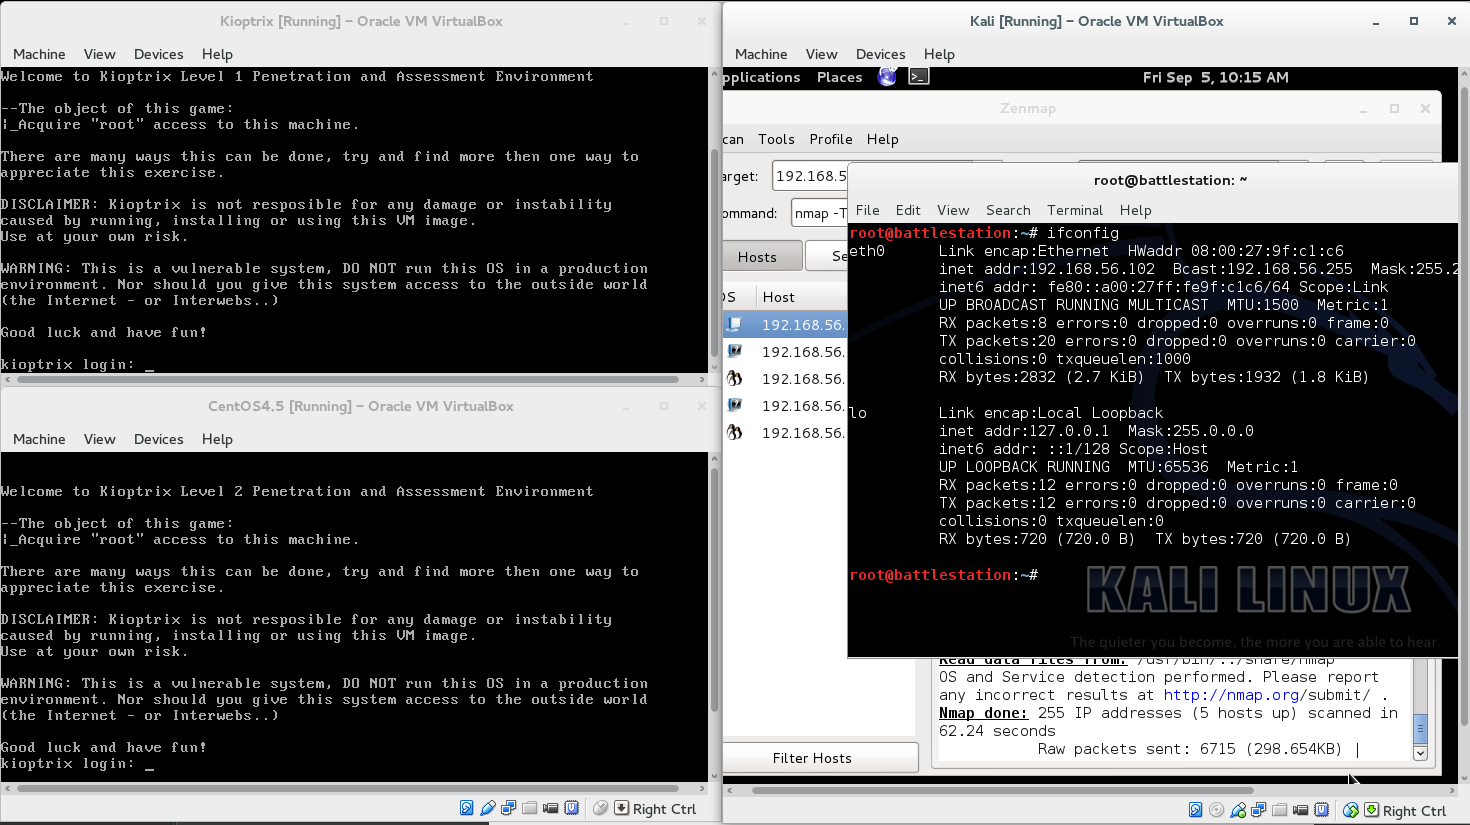
\includegraphics[scale=0.7]{ifconfig.png}

\section{Vulnerability report}
% Vuln report, OpenVAS
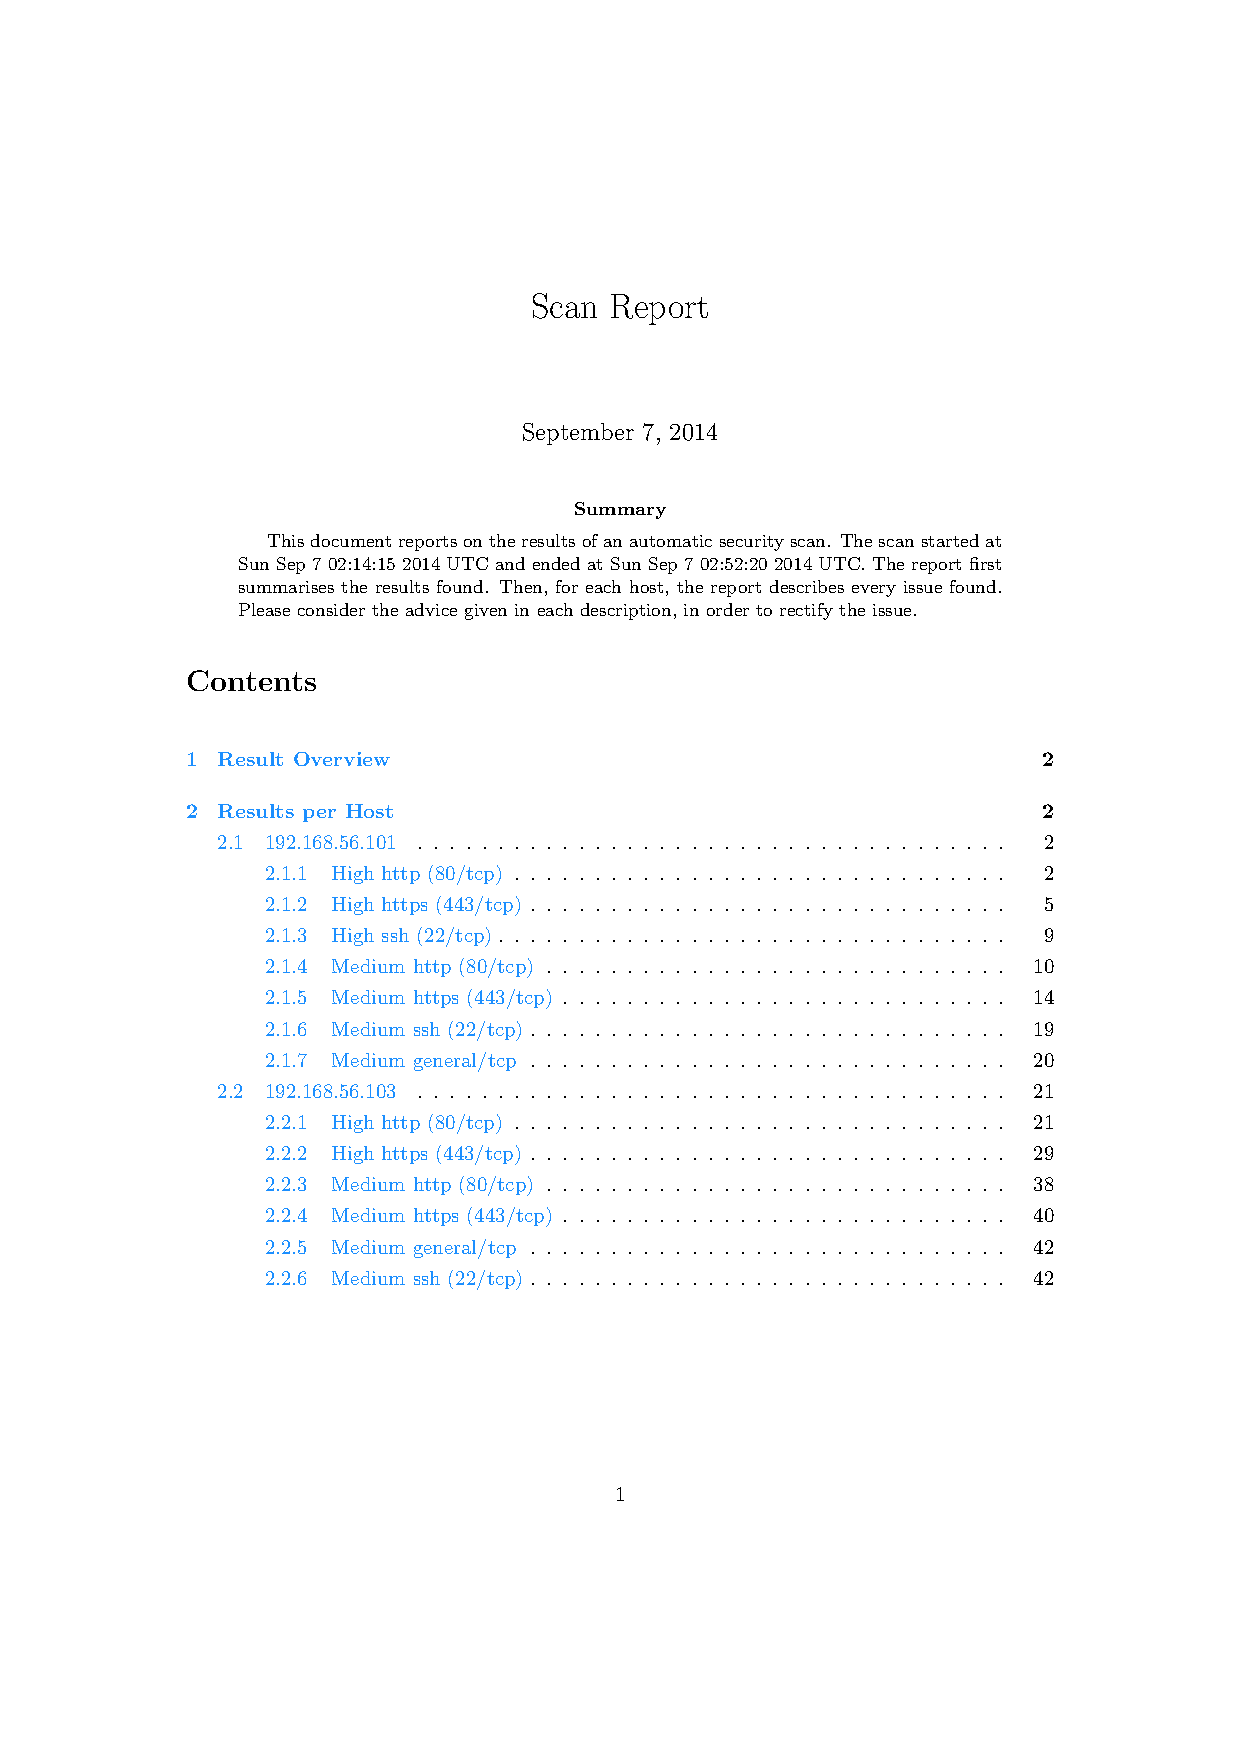
\includepdf[pages={-}]{vulns.pdf}
